\section{采用 JIT 优化的技能运行时}
\label{sec:runtime}

\begin{figure*}[t]
  \centering
  \setlength{\abovecaptionskip}{3pt}
  \setlength{\belowcaptionskip}{0pt}
  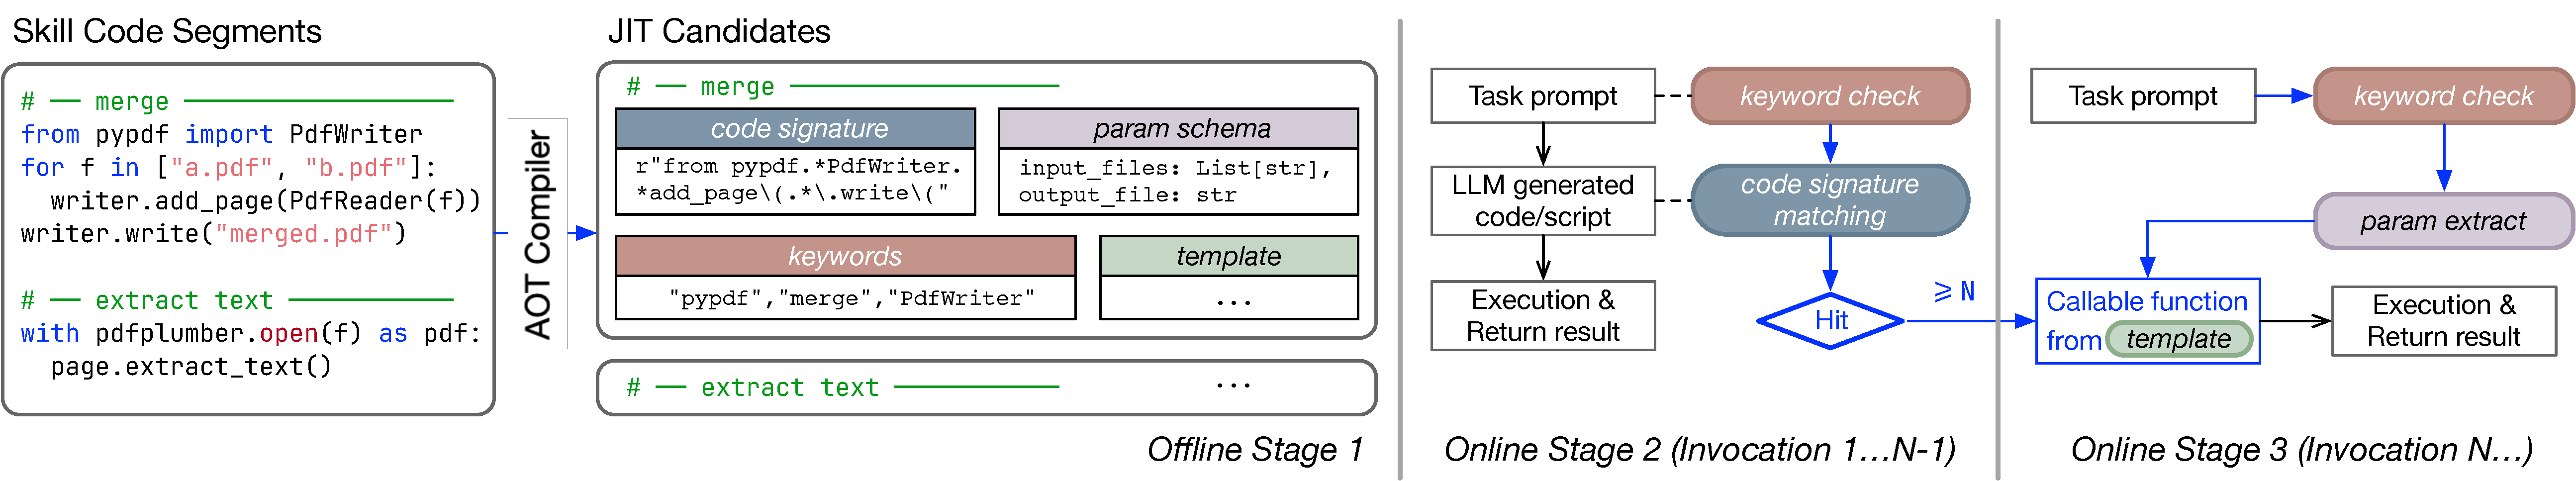
\includegraphics[width=\textwidth]{figures/code_solidification_pipeline.pdf}
  \caption{代码固化流水线。AOT 编译器分析技能中的代码段，并生成带代码签名与模板的 JIT 候选项（阶段~1）。运行时跨多次调用验证预测（阶段~2）。候选项晋升后，编译后的函数会替代 LLM 推理（阶段~3）。}
  \label{fig:solidification}
\end{figure*}

AOT 编译会为不同目标端生成多个技能变体。
因此在运行时，\sys 会加载为当前目标端编译的技能变体。
由于每个技能与目标端（模型+代理框架）组合只执行一次 AOT 编译，编译开销较小。

不过，有些问题只有到执行时才会浮现，例如静态画像遗漏的能力缺口，
或并行子代理争用受 API 速率限制约束的资源。
另一些机会，例如在多次调用中反复出现的代码模式，只有重复运行后才会显现。
\sys 运行时通过 JIT 优化（\S\ref{sec:runtime:jit}）和资源感知调度器（\S\ref{sec:runtime:sched}）处理这两类情况。

\subsection{技能注册与执行}
\label{sec:runtime:exec}

编译会为每个技能生成多个技能变体，以及阶段~2 生成的环境绑定脚本。
新任务到来时，运行时会选择为当前（模型，代理框架）组合编译的变体。
从代理的角度看，多个变体带来的复杂性是不可见的：
它看到的仍是一组技能，并通过 \S\ref{sec:insight} 所述的同一种渐进式披露机制加载它们。
在加载完整技能上下文之前，运行时会先执行环境绑定脚本，
验证运行时依赖是否已满足。

\subsection{JIT 优化}
\label{sec:runtime:jit}

AOT 编译会针对每个目标端调整原语能力；在此基础上，\sys 进一步应用 JIT 优化，
通过自适应重编译与代码固化这两种互补机制，
提高执行质量与效率。

\subsubsection{自适应重编译}
\label{sec:runtime:jit1}

运行时跟踪使用技能执行的每个任务的结果。
当技能执行失败（例如代理中止或收到人工反馈），或在代理循环中发生重试时，
运行时会记录结构化的失败或重试日志。
尽管当前模型可能通过反思进行自我纠正，
但纠正过程不会被记录，因此后续执行仍可能遇到相同错误。

当同一技能在多次调用中失败时，运行时会分析这些失败究竟是任务特有的，
还是反映技能本身存在系统性能力缺口。
只有后一种情况才会触发自适应重编译：
运行时把累积的失败日志和模型的自我恢复轨迹作为编译器输入，
由编译器对技能施加针对性的补偿变换。
如果重编译后的变体表现更差，运行时就回滚到前一版本。
后续每次重编译都从迄今观察到的最佳变体开始，
以确保优化能够改善技能性能。

\begin{figure*}[t]
  \centering
  \setlength{\abovecaptionskip}{0pt}
  \setlength{\belowcaptionskip}{0pt}
  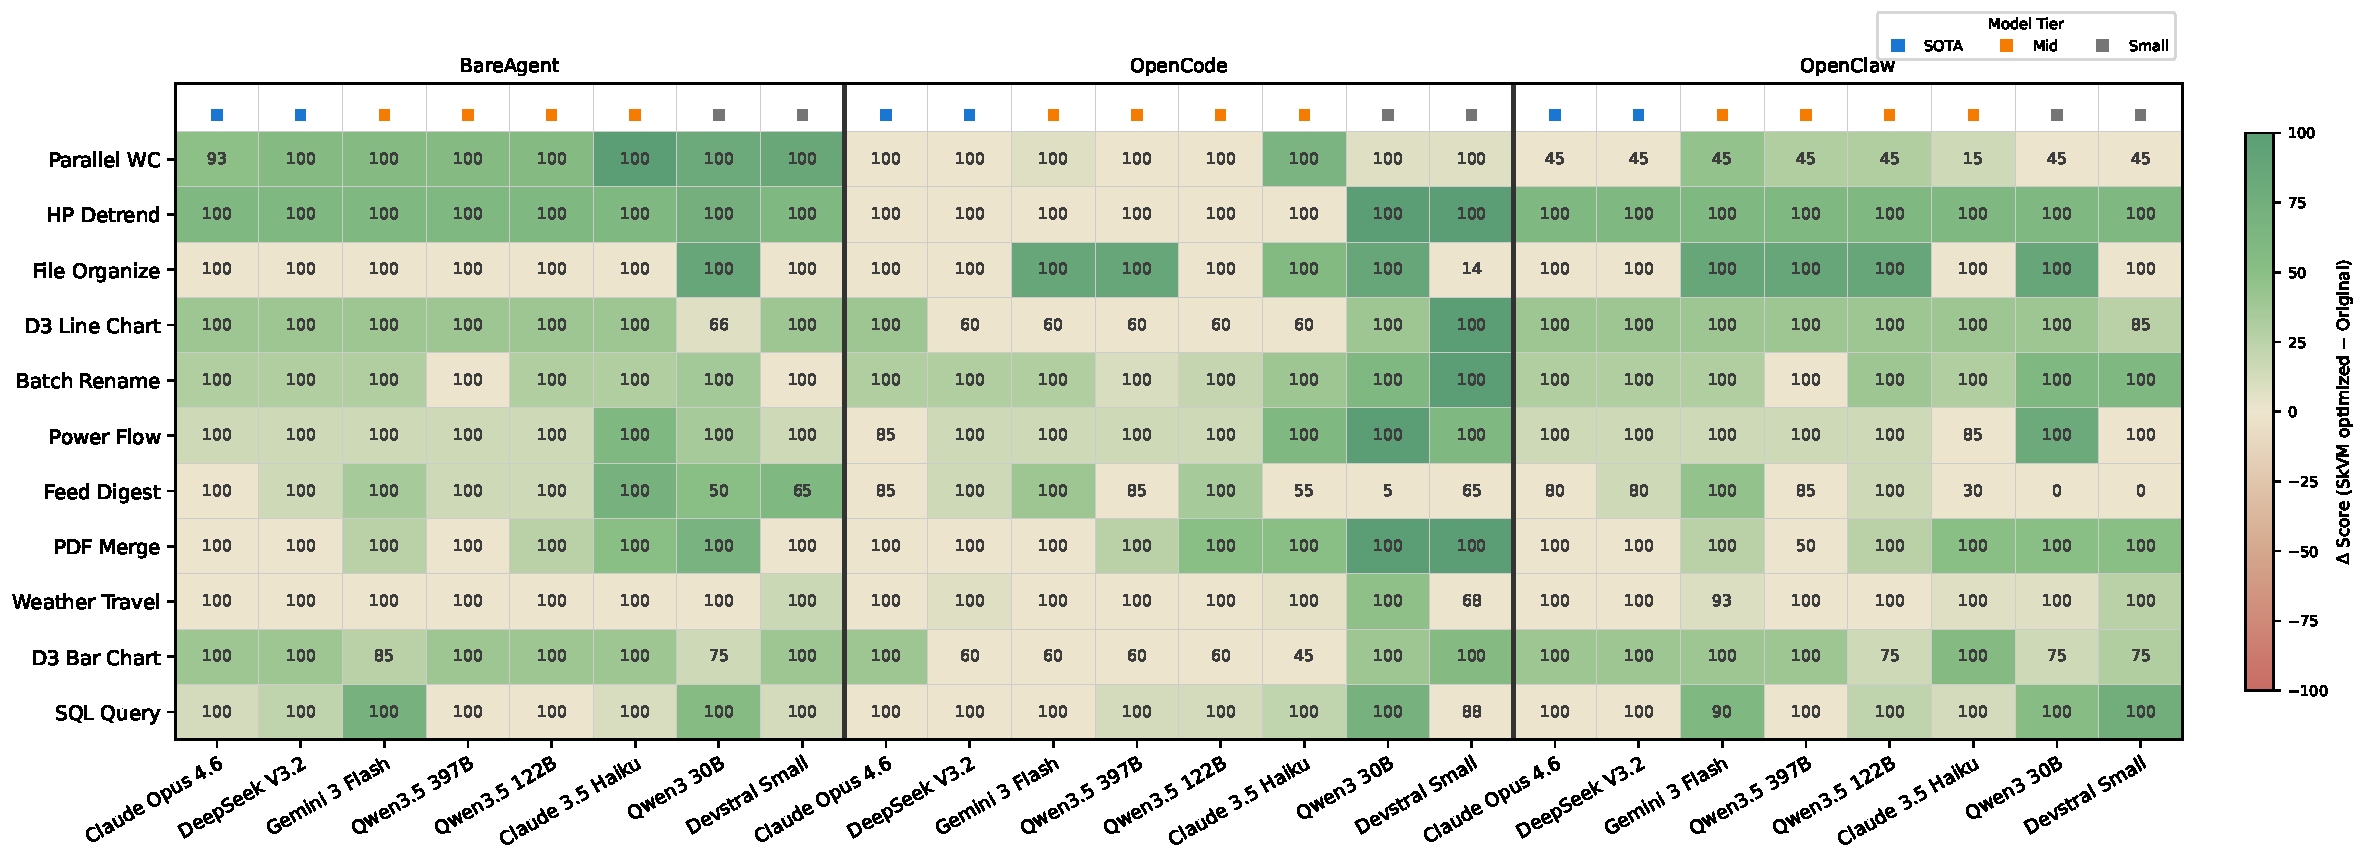
\includegraphics[width=\textwidth]{figures/e1_heatmap.pdf}
  \caption{技能编译的有效性。单元格数值表示经 \sys 优化后的任务完成率；单元格颜色表示相对于原始基线技能的分数提升（绿色）或下降（红色）。}
  \label{fig:e1_heatmap}
\end{figure*}

\subsubsection{代码固化}
\label{sec:runtime:jit2}
回顾前文，75\% 的技能包含可固化代码（\S\ref{sec:insight:analysis}）：
这类代码整体结构固定，只有输入相关参数发生变化。
在常规执行中，LLM 每次调用都会重新执行完整的推理和工具使用循环，
把 token 与延迟花在结构完全相同的过程上。
代码固化会识别这些重复模式，并将其晋升为绕过模型推理的可执行代码。
图~\ref{fig:solidification} 展示了包含三个阶段的流水线。

在第一阶段，AOT 编译器分析每个技能中的代码和脚本片段，
判断它们是否包含适合固化的参数化模式。
对于符合条件的片段，编译器会生成一个包含四部分的\emph{JIT 候选项}：
用于筛选相关调用的关键词；以匹配模式刻画预期输出结构的\emph{代码签名}；
带参数槽位的代码模板；以及描述可提取参数的参数模式。
这些候选项会与编译后的技能变体一同打包。

在第二阶段，运行时监控器观察多次重复调用中的 LLM 调用。
对于每次调用，它先检查关键词以判断相关性，再将生成的代码与代码签名匹配。
只有当代码签名在连续多次调用中成功匹配后，系统才会触发代码固化，
从而保证 LLM 生成的代码结构与 AOT 阶段分析出的模式保持一致。
如果模型输出持续偏离代码签名，系统会继续采用安全的 LLM 路径，绝不晋升该候选项。

在第三阶段，模板被实例化为可调用函数：
系统把模板代码与参数提取、输出处理封装在一起，生成独立的 shell 脚本或代码函数。
由于 AOT 阶段已经完成分析，这一步实例化轻量且机械化。
后续调用会完全绕过 LLM：运行时从任务上下文提取参数，调用实例化函数并返回结果。
如果固化代码的执行导致代理任务失败或遇到运行时异常，
\sys 会触发后备机制，重新启用基于 LLM 的代码生成以保证正确性。

\subsection{资源感知的并行调度}
\label{sec:runtime:sched}

在 AOT 编译的阶段~3 中，编译器会识别可能采用并行的位置；
但多大的并行度才\emph{高效}，取决于运行时不断变化的条件：
CPU 使用率、外部 API 速率限制、机器可用内存，以及其他共享资源。

\sys 动态监控系统状态并据此调度任务执行，
弥合编译时机会与运行时现实之间的差距。
对于受 API 约束的工作负载，它监控响应延迟与 HTTP 429（速率限制）信号；
对于计算密集型工作负载，它监控 CPU 与内存使用率。
当压力超过阈值时，\sys 会采用两种机制缓解资源争用。
首先，它对新子代理的启动实施节流，避免引入更多并发压力。
其次，对于已经运行的子代理，\sys 会根据每个代理的资源使用量或启动顺序，
有选择地挂起其中一部分（即暂停其代理循环执行），以减少对共享资源的活跃争用。
\sys 还会记录每个技能上次在当前系统运行时的有效并发度，并将其作为后续执行的并发提示。
